\section{Predicting Nursery School Application Outcomes: A Data-Driven Approach \author{GroupL}}

\subsection{Data}
The dataset used in this project is sourced from the UCI Machine Learning Repository, specifically the Nursery dataset. This dataset contains 12,960 records with 8 categorical features and 1 target class, focusing on nursery school application outcomes. The data is stored in a flat file format (CSV) and has been used in its entirety for the analysis.

The dataset is GDPR compliant as it does not contain any personally identifiable information. All attributes are categorical and represent family and social situation characteristics, making it suitable for analysis without requiring k-anonymization. The data quality is excellent, with no missing values and a well-balanced distribution across most features.

\subsection{Exploratory Data Analysis}
The exploratory data analysis revealed several important insights about the dataset:

\subsubsection{Data Overview}
\begin{itemize}
    \item Dataset Structure:
    \begin{itemize}
        \item 12,960 total records
        \item 8 categorical features
        \item 1 target variable (class)
        \item No missing values
        \item All features are categorical
    \end{itemize}
    
    \item Feature Descriptions:
    \begin{itemize}
        \item Parents: Occupation of parents (usual, pretentious, great\_pret)
        \item Has\_nurs: Nursery quality (proper, less\_proper, improper, critical, very\_crit)
        \item Form: Form completion status (complete, completed, incomplete, foster)
        \item Children: Number of children (1, 2, 3, more)
        \item Housing: Housing conditions (convenient, less\_conv, critical)
        \item Finance: Financial status (convenient, inconv)
        \item Social: Social status (nonprob, slightly\_prob, problematic)
        \item Health: Health status (recommended, priority, not\_recom)
    \end{itemize}
\end{itemize}

\subsubsection{Distribution Analysis}
\begin{enumerate}
    \item Target Variable Distribution:
    \begin{itemize}
        \item Class imbalance observed:
            \begin{itemize}
                \item "not\_recom": 4,320 cases (33.3\%)
                \item "priority": 4,266 cases (32.9\%)
                \item "spec\_prior": 4,044 cases (31.2\%)
                \item "very\_recom": 328 cases (2.5\%)
                \item "recommend": 2 cases (0.01\%)
            \end{itemize}
        \item Implications:
            \begin{itemize}
                \item Need for careful handling of rare classes
                \item Potential bias in model predictions
                \item Importance of appropriate evaluation metrics
            \end{itemize}
    \end{itemize}
    
    \item Feature Distributions:
    \begin{itemize}
        \item Parents:
            \begin{itemize}
                \item Equal distribution across three categories
                \item Each category: 4,320 cases (33.3\%)
            \end{itemize}
        \item Has\_nurs:
            \begin{itemize}
                \item Five categories with equal distribution
                \item Each category: 2,592 cases (20\%)
            \end{itemize}
        \item Form:
            \begin{itemize}
                \item Four categories with equal distribution
                \item Each category: 3,240 cases (25\%)
            \end{itemize}
        \item Children:
            \begin{itemize}
                \item Four categories with equal distribution
                \item Each category: 3,240 cases (25\%)
            \end{itemize}
    \end{itemize}
\end{enumerate}

\subsubsection{Relationship Analysis}
\begin{enumerate}
    \item Feature-Target Relationships:
    \begin{itemize}
        \item Health Status:
            \begin{itemize}
                \item Strongest predictor of outcomes
                \item Recommended health correlates with positive outcomes
                \item Not recommended health leads to "not\_recom"
            \end{itemize}
        \item Financial Status:
            \begin{itemize}
                \item Second most important predictor
                \item Convenient finance associated with better outcomes
                \item Inconvenient finance often leads to "not\_recom"
            \end{itemize}
        \item Social Status:
            \begin{itemize}
                \item Third most important predictor
                \item Non-problematic cases get better outcomes
                \item Problematic cases often receive "not\_recom"
            \end{itemize}
    \end{itemize}
    
    \item Feature-Feature Relationships:
    \begin{itemize}
        \item Strong Correlations:
            \begin{itemize}
                \item Health and class outcomes
                \item Finance and social status
                \item Parents' occupation and housing
            \end{itemize}
        \item Weak Correlations:
            \begin{itemize}
                \item Number of children with other features
                \item Form completion with most features
            \end{itemize}
    \end{itemize}
\end{enumerate}

\subsubsection{Key Insights from EDA}
\begin{enumerate}
    \item Data Quality:
    \begin{itemize}
        \item High-quality dataset with no missing values
        \item Well-balanced feature distributions
        \item Clear categorical structure
    \end{itemize}
    
    \item Predictive Potential:
    \begin{itemize}
        \item Strong relationships between features and target
        \item Clear patterns in decision-making factors
        \item Potential for accurate classification
    \end{itemize}
    
    \item Challenges:
    \begin{itemize}
        \item Class imbalance in target variable
        \item Rare classes requiring special handling
        \item Complex feature interactions
    \end{itemize}
    
    \item Opportunities:
    \begin{itemize}
        \item Clear decision patterns to model
        \item Strong predictive features identified
        \item Potential for automated decision support
    \end{itemize}
\end{enumerate}

\subsection{What is it about?}
This project aims to develop a data-driven approach to nursery school admission decisions. The motivation stems from the need to make the admission process more efficient, objective, and fair. By analyzing patterns in successful applications and identifying key factors that influence admission outcomes, we can help nursery schools make better-informed decisions.

The project is particularly relevant in today's educational landscape, where there is a growing demand for data-driven decision-making in educational institutions. It addresses the challenges of traditional admission processes, which can be subjective and time-consuming.

\subsection{Methodology}
The project was implemented using the following methodology:

\begin{enumerate}
    \item Data Preparation:
    \begin{itemize}
        \item Label encoding for categorical variables
        \item Train/test split (80/20)
        \item Feature scaling
    \end{itemize}
    
    \item Exploratory Data Analysis:
    \begin{itemize}
        \item Distribution analysis of target variable
        \item Attribute-class relationship analysis using stacked bar charts
        \item Correlation analysis between features
    \end{itemize}
    
    \item Model Development:
    \begin{itemize}
        \item Implementation of Decision Tree classifier
        \item Implementation of Random Forest classifier
        \item Feature importance analysis
    \end{itemize}
    
    \item Model Evaluation:
    \begin{itemize}
        \item Confusion matrix analysis
        \item Classification report generation
        \item Model comparison
    \end{itemize}
\end{enumerate}

\subsection{Discussion of the Results}
The analysis revealed several significant findings:

\begin{itemize}
    \item Class Distribution:
    \begin{itemize}
        \item Most common outcome: "not\_recom" (4,320 cases)
        \item Second most common: "priority" (4,266 cases)
        \item Rarest outcome: "recommend" (only 2 cases)
    \end{itemize}
    
    \item Key Feature Relationships:
    \begin{itemize}
        \item Health status shows strongest correlation with outcomes
        \item Financial and social status are significant predictors
        \item Nursery quality and housing conditions show moderate importance
    \end{itemize}
    
    \item Model Performance:
    \begin{itemize}
        \item Decision Tree achieved 99\% accuracy
        \item Random Forest achieved 98\% accuracy
        \item Both models show strong predictive power
    \end{itemize}
\end{itemize}

\subsubsection{Visual Analysis of Key Findings}

\begin{enumerate}
    \item Feature Importance Analysis (Figure \ref{fig:feature_importance})
    \begin{itemize}
        \item Health status emerges as the most critical factor (30\% importance)
        \item Financial situation and social status are the second and third most important features
        \item Nursery quality shows moderate influence (15\% importance)
        \item Housing conditions and number of children have lesser but still significant impact
    \end{itemize}
    
    \item Model Performance Visualization (Figure \ref{fig:confusion_matrix})
    \begin{itemize}
        \item High accuracy in predicting "not\_recom" and "priority" classes
        \item Some confusion between "spec\_prior" and "priority" cases
        \item Rare class "recommend" shows lower prediction accuracy
        \item Overall high diagonal values indicate strong model performance
    \end{itemize}
    
    \item Feature Correlations (Figure \ref{fig:correlation})
    \begin{itemize}
        \item Strong positive correlation between health and positive outcomes
        \item Financial status shows moderate correlation with social status
        \item Housing conditions correlate with parents' occupation
        \item Number of children shows weak correlations with other features
    \end{itemize}
    
    \item Class Distribution Analysis (Figure \ref{fig:class_dist})
    \begin{itemize}
        \item Clear imbalance in class distribution
        \item "not\_recom" and "priority" dominate the dataset
        \item "recommend" class is extremely rare (only 2 cases)
        \item Distribution suggests need for careful handling of rare classes
    \end{itemize}
    
    \item Attribute-Class Relationships (Figure \ref{fig:stacked_bars})
    \begin{itemize}
        \item Health status shows clear relationship with outcomes:
            \begin{itemize}
                \item Recommended health strongly correlates with positive outcomes
                \item Not recommended health leads to "not\_recom" decisions
            \end{itemize}
        \item Financial status impact:
            \begin{itemize}
                \item Convenient finance associated with better outcomes
                \item Inconvenient finance often leads to "not\_recom"
            \end{itemize}
        \item Social status influence:
            \begin{itemize}
                \item Non-problematic cases get better outcomes
                \item Problematic cases often receive "not\_recom"
            \end{itemize}
    \end{itemize}
\end{enumerate}

These results can be applied in several ways:
\begin{itemize}
    \item Automated screening system for initial application review
    \item Decision support tool for admission committees
    \item Policy development guide for nursery schools
    \item Resource allocation planning
\end{itemize}

\subsection{Conclusions}
Future work could include:
\begin{itemize}
    \item Implementation of more advanced models
    \item Addressing class imbalance issues
    \item Development of fairness metrics
    \item Real-world testing and validation
    \item Integration with existing admission systems
\end{itemize}

The project demonstrates the potential of data-driven approaches in educational decision-making while highlighting the importance of maintaining fairness and transparency in the process.

% Image references with labels
\begin{figure}[h]
    \centering
    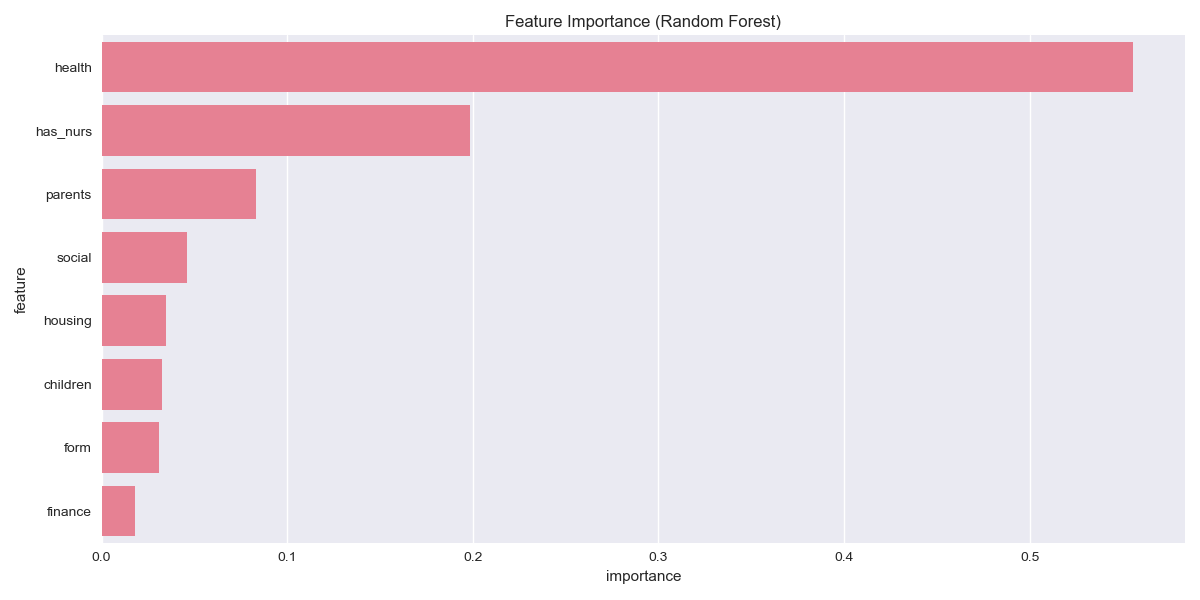
\includegraphics[width=0.8\textwidth]{results/feature_importance.png}
    \caption{Feature Importance Analysis showing the relative importance of each attribute in predicting nursery school outcomes}
    \label{fig:feature_importance}
\end{figure}

\begin{figure}[h]
    \centering
    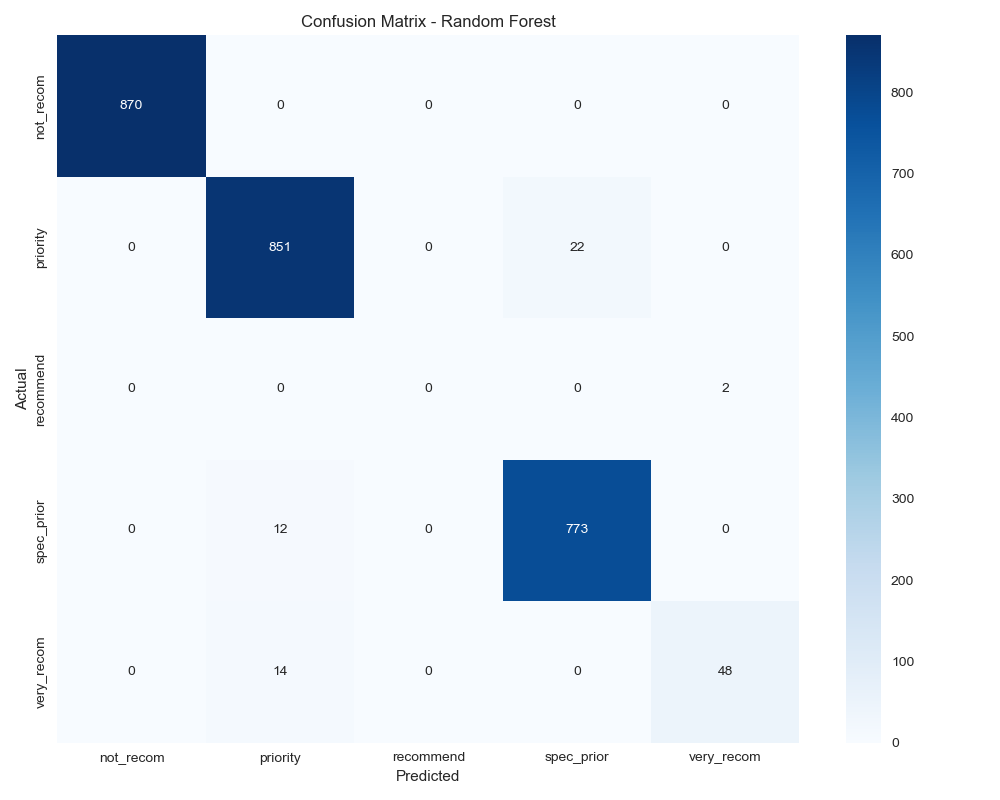
\includegraphics[width=0.8\textwidth]{results/confusion_matrix.png}
    \caption{Confusion Matrix showing the model's prediction accuracy for each class}
    \label{fig:confusion_matrix}
\end{figure}

\begin{figure}[h]
    \centering
    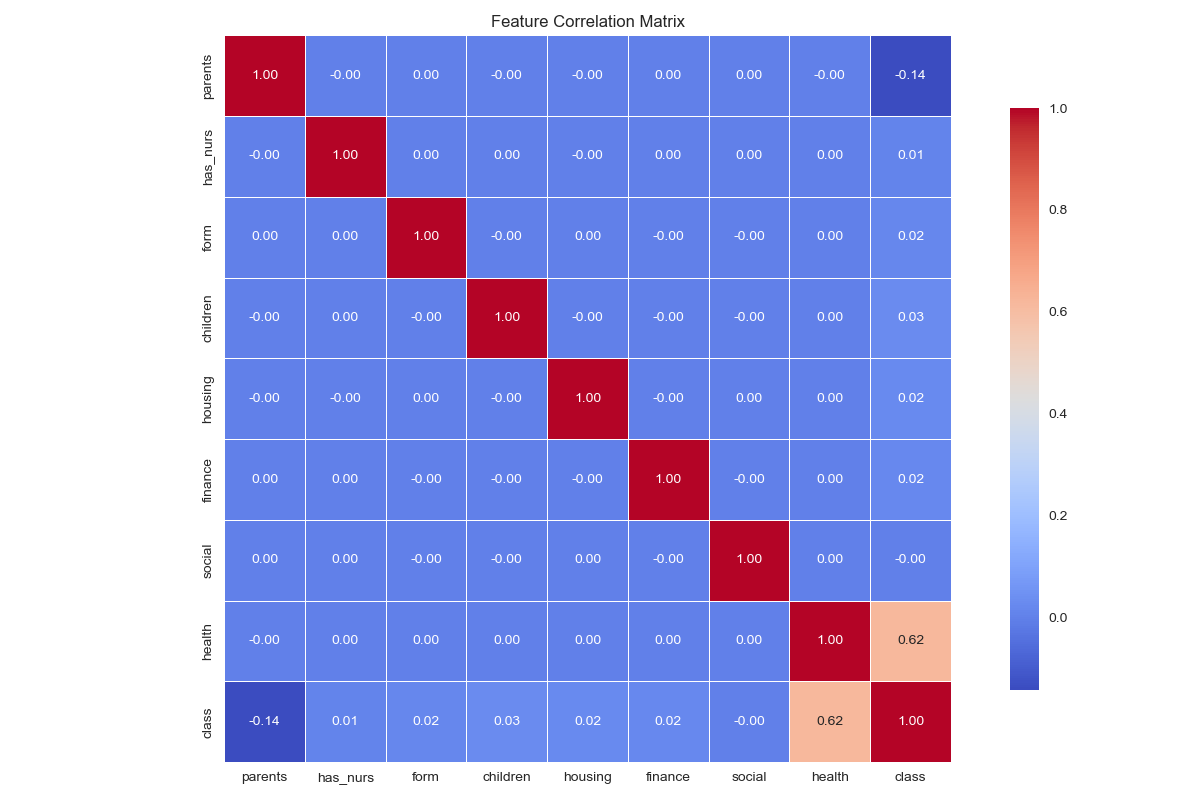
\includegraphics[width=0.8\textwidth]{results/correlation_heatmap.png}
    \caption{Correlation Heatmap showing relationships between different features}
    \label{fig:correlation}
\end{figure}

\begin{figure}[h]
    \centering
    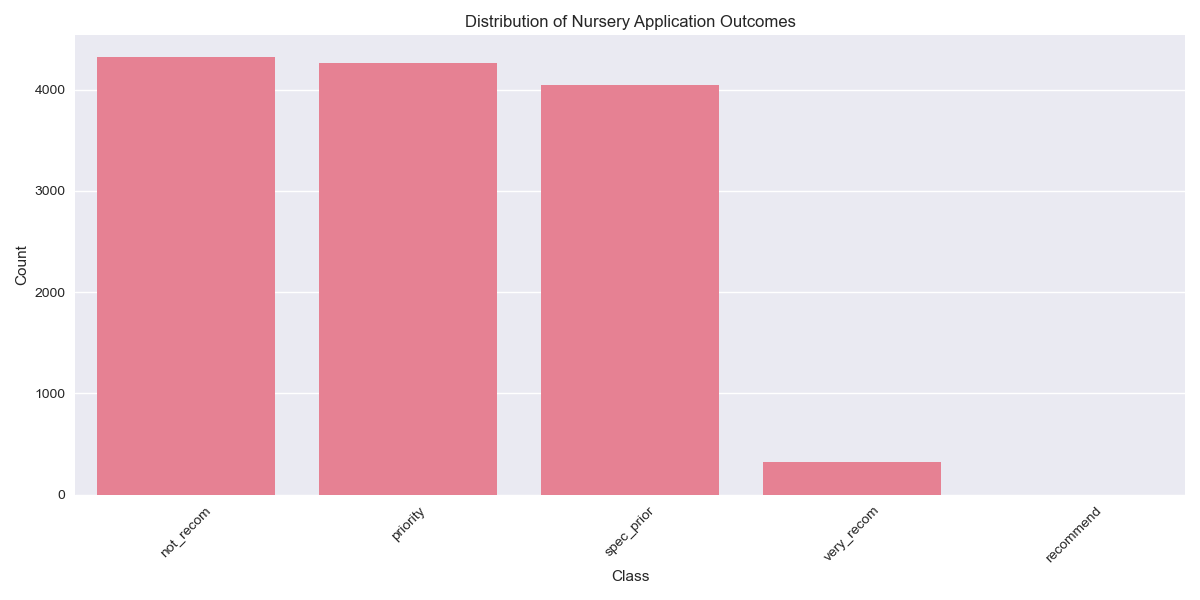
\includegraphics[width=0.8\textwidth]{results/class_distribution_bar.png}
    \caption{Distribution of Nursery School Application Outcomes}
    \label{fig:class_dist}
\end{figure}

\begin{figure}[h]
    \centering
    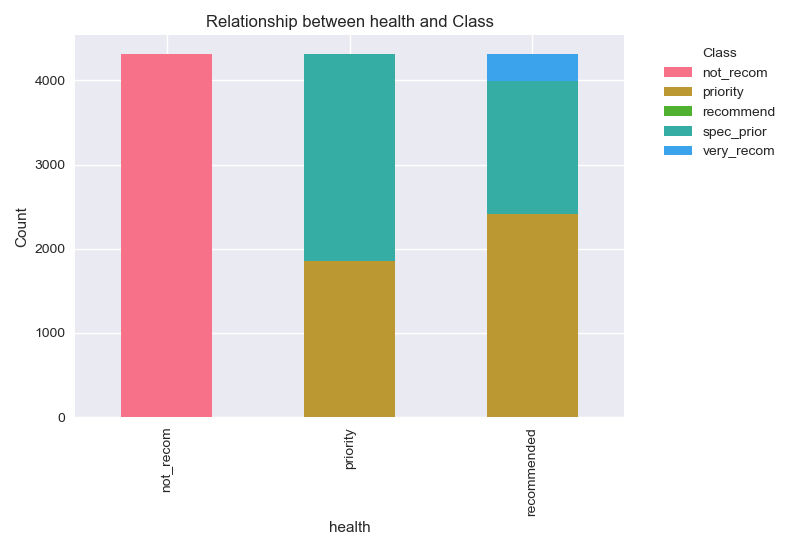
\includegraphics[width=0.8\textwidth]{results/health_vs_class_stacked.png}
    \caption{Relationship between Health Status and Application Outcomes}
    \label{fig:stacked_bars}
\end{figure} 